% This is "sig-alternate.tex" V2.0 May 2012
% This file should be compiled with V2.5 of "sig-alternate.cls" May 2012
%
% This example file demonstrates the use of the 'sig-alternate.cls'
% V2.5 LaTeX2e document class file. It is for those submitting
% articles to ACM Conference Proceedings WHO DO NOT WISH TO
% STRICTLY ADHERE TO THE SIGS (PUBS-BOARD-ENDORSED) STYLE.
% The 'sig-alternate.cls' file will produce a similar-looking,
% albeit, 'tighter' paper resulting in, invariably, fewer pages.
%
% ----------------------------------------------------------------------------------------------------------------
% This .tex file (and associated .cls V2.5) produces:
%       1) The Permission Statement
%       2) The Conference (location) Info information
%       3) The Copyright Line with ACM data
%       4) NO page numbers
%
% as against the acm_proc_article-sp.cls file which
% DOES NOT produce 1) thru' 3) above.
%
% Using 'sig-alternate.cls' you have control, however, from within
% the source .tex file, over both the CopyrightYear
% (defaulted to 200X) and the ACM Copyright Data
% (defaulted to X-XXXXX-XX-X/XX/XX).
% e.g.
% \CopyrightYear{2007} will cause 2007 to appear in the copyright line.
% \crdata{0-12345-67-8/90/12} will cause 0-12345-67-8/90/12 to appear in the copyright line.
%
% ---------------------------------------------------------------------------------------------------------------
% This .tex source is an example which *does* use
% the .bib file (from which the .bbl file % is produced).
% REMEMBER HOWEVER: After having produced the .bbl file,
% and prior to final submission, you *NEED* to 'insert'
% your .bbl file into your source .tex file so as to provide
% ONE 'self-contained' source file.
%
% ================= IF YOU HAVE QUESTIONS =======================
% Questions regarding the SIGS styles, SIGS policies and
% procedures, Conferences etc. should be sent to
% Adrienne Griscti (griscti@acm.org)
%
% Technical questions _only_ to
% Gerald Murray (murray@hq.acm.org)
% ===============================================================
%
% For tracking purposes - this is V2.0 - May 2012

\documentclass{sig-alternate}

\usepackage{url}

\begin{document}
%
% --- Author Metadata here ---
\conferenceinfo{Workshop on the theory and practice of social machines @ WWW2013}{2013, Rio de Janeiro, Brazil}
%\CopyrightYear{2007} % Allows default copyright year (20XX) to be over-ridden - IF NEED BE.
%\crdata{0-12345-67-8/90/01}  % Allows default copyright data (0-89791-88-6/97/05) to be over-ridden - IF NEED BE.
% --- End of Author Metadata ---

\title{Towards a classification framework for social machines}
%\subtitle{[Extended Abstract]
%\titlenote{A full version of this paper is available as
%\textit{Author's Guide to Preparing ACM SIG Proceedings Using
%\LaTeX$2_\epsilon$\ and BibTeX} at
%\texttt{www.acm.org/eaddress.htm}}}
%
% You need the command \numberofauthors to handle the 'placement
% and alignment' of the authors beneath the title.
%
% For aesthetic reasons, we recommend 'three authors at a time'
% i.e. three 'name/affiliation blocks' be placed beneath the title.
%
% NOTE: You are NOT restricted in how many 'rows' of
% "name/affiliations" may appear. We just ask that you restrict
% the number of 'columns' to three.
%
% Because of the available 'opening page real-estate'
% we ask you to refrain from putting more than six authors
% (two rows with three columns) beneath the article title.
% More than six makes the first-page appear very cluttered indeed.
%
% Use the \alignauthor commands to handle the names
% and affiliations for an 'aesthetic maximum' of six authors.
% Add names, affiliations, addresses for
% the seventh etc. author(s) as the argument for the
% \additionalauthors command.
% These 'additional authors' will be output/set for you
% without further effort on your part as the last section in
% the body of your article BEFORE References or any Appendices.

\numberofauthors{1} %  in this sample file, there are a *total*
% of EIGHT authors. SIX appear on the 'first-page' (for formatting
% reasons) and the remaining two appear in the \additionalauthors section.
%
\author{
% You can go ahead and credit any number of authors here,
% e.g. one 'row of three' or two rows (consisting of one row of three
% and a second row of one, two or three).
%
% The command \alignauthor (no curly braces needed) should
% precede each author name, affiliation/snail-mail address and
% e-mail address. Additionally, tag each line of
% affiliation/address with \affaddr, and tag the
% e-mail address with \email.
%
% 1st. author
\alignauthor
Authors\\
       \affaddr{Web and Internet Science Group}\\
       \affaddr{University of Southampton}\\
       \affaddr{Southampton, UK}\\
       \email{\{a,b,c,d,wh,nrs\}@ecs.soton.ac.uk}
}
% There's nothing stopping you putting the seventh, eighth, etc.
% author on the opening page (as the 'third row') but we ask,
% for aesthetic reasons that you place these 'additional authors'
% in the \additional authors block, viz.
%\additionalauthors{Additional authors: John Smith (The Th{\o}rv{\"a}ld Group,
%email: {\texttt{jsmith@affiliation.org}}) and Julius P.~Kumquat
%(The Kumquat Consortium, email: {\texttt{jpkumquat@consortium.net}}).}
%\date{30 July 1999}
% Just remember to make sure that the TOTAL number of authors
% is the number that will appear on the first page PLUS the
% number that will appear in the \additionalauthors section.

\maketitle
\begin{abstract}

This paper provides a framework for...

\end{abstract}

% A category with the (minimum) three required fields
%\category{H.4}{Information Systems Applications}{Miscellaneous}
%A category including the fourth, optional field follows...
%\category{D.2.8}{Software Engineering}{Metrics}[complexity measures, performance measures]

%\terms{Theory}

%\keywords{ACM proceedings, \LaTeX, text tagging}

\section{Social machines: an introduction}
Once upon a time 'machines' were programmed by programmers and used by users. The success of the Web has changed this relationship: we now see configurations of people interacting with content and with each other, typified by social Web sites. Rather than drawing a line through such Web-based systems to separate the human and machine parts (as Computer Science has traditionally done), we can now draw a line around them  and  treat  each  such  assembly  as  a  'social  machine'  -  a  machine  in which  digital  and  human components are seamlessly interwoven. This crucial transition in thinking acknowledges the reality of current socio-technical systems, and is essential to underpin any understanding of the science and engineering of their future development towards pervasive ecosystems of co-evolving social machines.

A number of prominent examples aside, today we still see a divide between conventional IT systems dedicated to data- and computation-intensive tasks, and Web $2.0$ sites offering some combination of well-known participatory features, in which user-generated content and the underlying social network evolve dynamically and hand-in-hand. As technology becomes more and more ubiquitous, many of the challenges we will witness in any domain of our life, business, and society will need solutions that rely on both of these axes: a sophisticated  combination  of  data-intensive, complex automation and deep community involvement. This suggests the need for new types of systems to tackle these challenges, and to achieve requires a through understanding of the science and engineering of social machines.

As a first step, we propose a classification framework for social machines, which can be used to describe, study, and compare this expanding field of interdisciplinary research and the increasing number of systems combining human and computational intelligence to serve purposes as diverse as traffic management, healthcare, media and journalism, or design and natural sciences.

In this paper we introduce the current version of the framework, which is the result of a knowledge elicitation process performed internally in our lab. Our aim is to present it to the broader community and extend and revise it based on their feedback in order to achieve a shared understanding, terminology, and set of descriptive features to enable a systematic study of existing and future social machines. Using a common descriptive classification allows researchers to observe the effects of specific technical properties of a system on social behavior, identify design and evolution patterns, learn about social network formation and dynamics, and devise incentive mechanisms to encourage large-scale participation. A second audience group targeted by our work are developers of social machines. For them, the framework may provide a theoretical grounding for the realization of new systems, informing system design and operation in terms of critical features and predicted user behavior and community development.

\section{What are social machines?}
Social machines can be basically characterized as assemblies of human and automatic components and their interaction. A  traditional  database,  with  users  looking  up  records  independently  of  each  other  and  an  administrator responsible for content, has some of the right ingredients but there is really no social component in this strict provider-consumer relationship. When we fill out a form (e.g., health information, birds spotted in my garden) it  is minimally  a  social machine  because humans  are  part  of  the  'social  computation'.  This  becomes  richer when  the database  is  curated by members  of  the  community  (e.g., Wikipedia) and when  the  social network adds value implicitly (Amazon) or explicitly (Facebook). We anticipate many categories of social machine in this continuum, and they may manifest themselves as Web site or app, or indeed in the Internet of Things.

To describe social machines we roughly rely on four different categories of classification features:

\begin{description}
  \item [The types of tasks undertaken by the social component and the resulting contributions]: social machines, just as any computing system, are built with a given purpose in mind, and exhibit functionality by which this purpose can be achieved. Users and the emerging social network interact with the system and with each other to carry out specific tasks by which they contribute to the 'computation'. This includes the creation and refinement of digital artifacts by executing given actions, possibly in collaboration with other participants. For example, in GalaxyZoo\footnote{\url{http://www.galaxyzoo.org}} people classify galaxies with collective performance as good as professional astronomers, while in reCaptcha\footnote{\url{http://www.google.com/recaptcha}} they refine the data that describes digital manuscripts. Sometimes, systems look for innovative ways of getting people to engage with the systems, including game narratives, like in EteRNA\footnote{\url{http://eterna.cmu.edu}}, in which  participants design RNA  that is evaluated automatically using simulators and then refined via human effort, or monetary rewards, like in Amazon's Mechanical Turk, a platform in which users undertake routine (micro) tasks such as object classification, audio transcription and text translation.

  \item [The roles of the participants and the social network they form]:

  \item [The motivating factors and incentive mechanisms]: system features influencing user behavior and the social network dynamics

  \item [Interaction between social and machine component]: how are human contributions used to compute things, including quality control, spam, workflow, aggregation of results
\end{description}


\section{Comparison with related fields}

A Social Machine includes human and machine two major components, therefore the study of social machine is an interdisciplinary endeavour. Since the Turning machine was invented, there has been a `paradigm shift' \cite{kuhn1996structure} in using computers, where the computer facilitates human communication rather acts as a purely calculative device. The Computer-supported Collaboration Work (CSCW) \cite{grudin1994computer} emerged in 1984 represents such shift. It addresses ``how collaborative activities and their coordination can be supported by means of computer systems''. This concept later evolved into a broader sense of  Computer-supported collaboration (CSC). The Social computing \cite{parameswaran2007research} is another shift, which refers systems that support ``the gathering, representation, processing, use, and dissemination of information that is distributed across social collectivities such as teams, communities, organizations, and markets''. To compare with the CSC, the social computing has more focus in `computing' rather than `collaboration'. Similarly, the Human Computation \cite{von2009human} is another paradigm towards the computational direction, which utilize human processing power to solve problems that computers cannot yet solve. All these three mentioned fields overlap in their concepts and are mainly popularised in the computer science. In the Web 2.0 era, there were few generic concepts/buzzword emerged on the idea of utilising the human power which are not only used in computer science, but also in other fields such as social science, business etc. Crowding sourcing \cite{howe2006crowdsourcing} as an example, describes the idea that taking a job traditionally performed by a designated agent and outsourcing it to an undefined, generally large group of people in the form of an open call. Open Innovation \cite{chesbrough2008open} advocates the similar idea with empathizing on the innovation in firms. Surowiecki also argued in the book of the wisdom of crowds \cite{surowiecki2005wisdom} that the aggregation of information in groups, resulting in decisions that are often better than could have been made by any single member of group. Collective Intelligence described by Malone \cite{malone2009harnessing}, defines an even more broadly concept that ``groups of individuals doing things collectively that seem intelligent.''
The concept overlapping between human computation, crowdsourcing, social computing and collective intelligence is discussed in \cite{quinn2011human}.
In  social machines  the  social and  the  technical are equal  partners. While  crowdsourcing  could  be  viewed  as  'human  subroutines'  and  'citizen  sensors',  the social machine perspective is one of incentivised participation and not humans enslaved to computers. We define the scope of social machine in a venn digram in Figure \ref{socialmachine}.

The study of social machines is naturally an interdisciplinary endeavor. Since the Turning machine was invented, we have experienced a paradigm shift in computer science from computers as purely calculative devices into a worldwide interconnected computer infrastructure which facilitates almost any type of human endeavor. The Computer-supported Collaboration Work (CSCW) \cite{grudin1994computer} emerged in 1984 represents such shift. It addresses ``how collaborative activities and their coordination can be supported by means of computer systems''. This concept later evolved into a broader sense of  Computer-supported collaboration (CSC). The Social computing \cite{parameswaran2007research} is another shift, which refers systems that support ``the gathering, representation, processing, use, and dissemination of information that is distributed across social collectivities such as teams, communities, organizations, and markets''. To compare with the CSC, the social computing has more focus in `computing' rather than `collaboration'. Similarly, the Human Computation \cite{von2009human} is another paradigm towards the computational direction, which utilize human processing power to solve problems that computers cannot yet solve. All these three mentioned fields overlap in their concepts and are mainly popularised in the computer science. In the Web 2.0 era, there were few generic concepts/buzzword emerged on the idea of utilising the human power which are not only used in computer science, but also in other fields such as social science, business etc. Crowding sourcing \cite{howe2006crowdsourcing} as an example, describes the idea that taking a job traditionally performed by a designated agent and outsourcing it to an undefined, generally large group of people in the form of an open call. Open Innovation \cite{chesbrough2008open} advocates the similar idea with empathizing on the innovation in firms. Surowiecki also argued in the book of the wisdom of crowds \cite{surowiecki2005wisdom} that the aggregation of information in groups, resulting in decisions that are often better than could have been made by any single member of group. Collective Intelligence described by Malone \cite{malone2009harnessing}, defines an even more broadly concept that ``groups of individuals doing things collectively that seem intelligent.''
The concept overlapping between human computation, crowdsourcing, social computing and collective intelligence is discussed in \cite{quinn2011human}.
In  social machines  the  social and  the  technical are equal  partners. While  crowdsourcing  could  be  viewed  as  'human  subroutines'  and  'citizen  sensors',  the social machine perspective is one of incentivised participation and not humans enslaved to computers. We define the scope of social machine in a conceptual digram in Figure \ref{socialmachine}.

\begin{figure}[htb]
\begin{center}
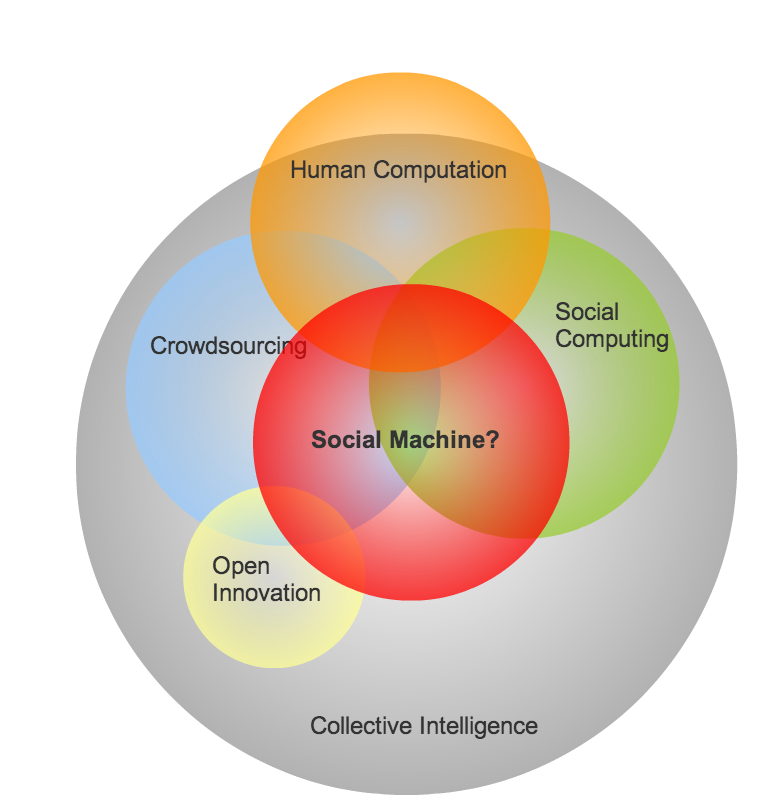
\includegraphics[width=8cm]{img/socialmachinescope.png}
\caption{Social machines and related areas} \label{social machine}
\end{center}
\end{figure}

\section{Classification of social machines}

\subsection{Methodology}

The classification framework presented in this paper was created through knowledge elicitation ~\cite{knowledgeelicitation}. In particular we used the {\it repertory grid} elicitation
technique~\cite{kelly} in order to derive an initial set of {\it elements}, which represent instances of social machines, and {\it constructs}, which capture their most important characteristics.

In repertory grid elicitation a software tool is used to ask users to describe constructs
that differentiate between elements - for example,  prompting the user to create a construct that
differentiates between {\it GalaxyZoo} and {\it Facebook}, as two prominent example of social machines our classification framework should apply to. The user describes the opposing poles of the construct - in this case, the user may decide on 'For Science' and 'For Socialising' in order to capture the core distinction between the two system. The user then rates every element with value from $1$ to $5$ on this construct, where $1$ represents an element that is purely
'For Science', and $5$ one that mainly serves  'socialising' purposes. Elements can also be rated with values between the poles if they may correspond to both or neither. The repertory grid software then identifies elements that are the least differentiated when requesting new constructs, in an attempt to elicit as much knowledge as possible from the user. We applied this technique to create an initial set of examples of social machines and to classify them according to specific features. To do so, we asked then computer science researchers familiar with the field to create their own repertory grids, and populate the elements from their own knowledge, and created the constructs using the standard repertory grid elicitation technique described above. This exercise led to $10$ grids, the union of which comprised a total of $56$ unique elements (social machines)
and $117$ different constructs (classifying factors). As the aim of this initial phase was to understand how people perceive the notion of social machine and their most distinctive properties, we allowed the participants to choose the social machines they are familiar with and describe them in their own terms.

%To enrich the resulting list of classifying constructs we then extracted the most frequent tags used in connection to the $56$ systems mentioned by the participants from the online bookmarking service {\it delicious.com}, thus achieving a crowdsourced social-machine classification containing the following clusters: Social Networks, (Micro)Blogging, News Aggregators, Image Boards, Crowd Science, Answer Gardens, Community Watch, Health and Wellbeing Support, Action and Investigation, Opinion Sharing, Video Sharing, Photo Sharing, Code Sharing, Art Sharing, Crowdsourcing Platforms, Mash-up Systems, and Crowdsourcing Toolkits and Platforms.

While determining the intersection of elements was straightforward, the consolidation of the
constructs required a more thorough process. We embarked on a manual process of grouping the constructs into rough clusters, based around the areas they cover. For example, we used construct
clusters including: Users, Motivation, Popularity, Technology, and Purpose. We then examined
each construct to determine which were equivalent, and whether we could re-word or subsume
existing constructs to cover the same aspects as a construct, with the aim to remove any
redundancy, to cut the list of constructs down to a manageable number, but to ensure that
all of the constructs that were elicited were somehow represented in the final set. This
process involved four of the authors discussing the choices, and finally agreeing on a
consolidated set of $31$ constructs.

%Even with this reduced set of constructs, if a single person were to classify all 56
%elements, this would still require 1736 individual decisions, and hence is unfeasible to
%expect full coverage of the elements using all of these constructs, despite how representative
%they are.
%
%[something here about doing 2 grids each and verifying the results?]
%
%To extract greater usefulness, and the ability to use our constructs to classify social
%machines we re-evaluated the constructs and the semantics that they represent into richer
%constructs that are not constrained by the 1-5 rating of repertory grid constructs.

\subsection{Classification dimensions}

\subsubsection{The polyarchical relationship of social machines}
While determining a set of social machines, one clear distinction was between social machine frameworks, such as MediaWiki and Ushahidi, which enable
social machines to be created, and instantiations of those frameworks into social machines that have been created for a specific purpose, such as Wikipedia
and Ushahidi Haiti. However, through further investigation, we discovered that the distinction between framework and instantiations was not the only
differentiator. Specifically, that some social machines could also have sub-machines or communities within them, that are working to solve different problems,
within the context of the larger machine. For example, Wikipedia is an instantiation of the MediaWiki framework, but there are a large number of
communities within Wikipedia that work on domain-specific areas, such as those contributing in areas of science and technology\footnote{Visualisation of Wikipedia Science Communities: \url{http://www.olihb.com/WikiCommunities/}}. However, we must also note that wikipedia is primarily split into communities of language, with the English, German and French wikipedias having the largest number of articles. It is therefore possible to analyse wikipedia into a hierarchy, from MediaWiki, to the languages of Wikipedia, down to the domain-specific communities. We explored this idea further, to include other social machines, and links where social machines utilise other social machines in order to function. For example, the social machine used by the Obama '12 US Presidential campaign~\cite{obamakieron}, which relied on social machines such as Twitter and Facebook.

Looking at the set of social machines in a polyarchy leads to a broad/specific relationship emerging that lets us talk about behaviours at various levels of granularity.  We propose looking at nested machines with ``The Web'' as one of several potential roots, with the next level down consisting of sub-platforms (such as Facebook, Twitter, MediaWiki, Ushahidi platforms) that spawn more specific social machines. A resulting polyarchy is shown in Figure~\ref{polyarchy}, which classifies levels as Infrastructure, Frameworks, Services and Causes/Groups.

\begin{figure}[htb]
\begin{center}
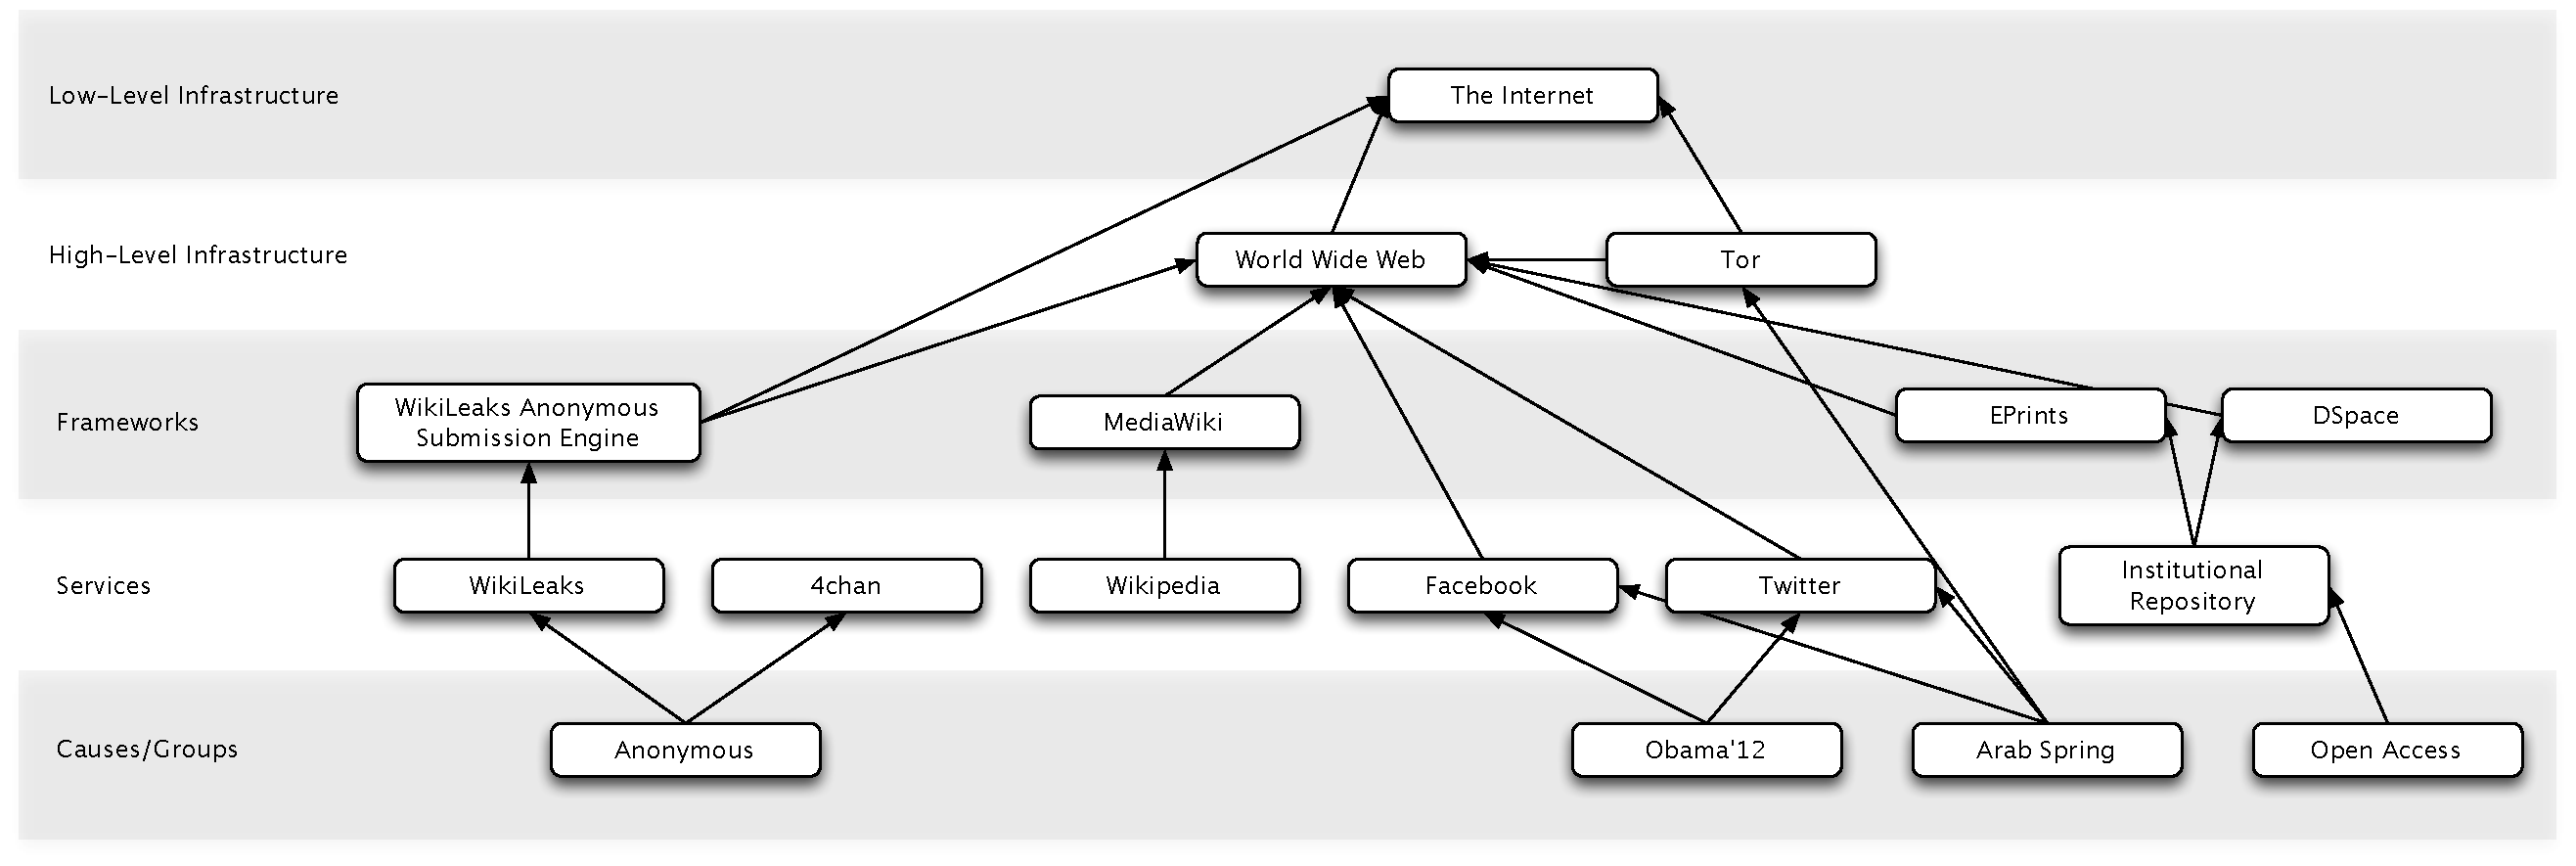
\includegraphics[width=8.5cm]{img/polyarchy.pdf}
\caption{A polyarchy of Social Machines, illustrating the infrastructure and frameworks used by social machines, and machine-machine usage.} \label{polyarchy}
\end{center}
\end{figure}

This approach enables us to start with a more detailed analysis of certain levels over others;
and seeing what similarities flow up and down the polyarchy. For example, what do
specific instances of Ushahidi/Zooniverse/MediaWiki have in common with other instances, and
how to they differ dynamically?

One originally unforeseen classification is that of the causes that utilise Social Machines.
Through a particularly popular cause, large numbers of participants can be mobilised, for
either a short period of time, or for long-term engagement, using multiple social machines
in order to further their cause. Examples of causes can be seen in Figure~\ref{polyarchy},
at the lowest level of the polyarchy. One such example is the cause of ``Open Access'' to
academic publications~\cite{harnad2001self}. This cause mobilises academic authors to
self-archive their own papers online so they are available for free, in addition to hosted
versions behind publishers pay-walls. In order to achieve this aim, the social machine of
``open access'' typically uses the social machines of institutional repositories provided
by the authors' associated institutions. As with other social machines, these social
machines typically use off-the-shelf implementations (in this case the most popular are
EPrints~\cite{eprints} and DSpace~\cite{dspace}), which run as web sites on the world wide
web. This cause is mature, growing year-on-year and has global coverage.

\subsubsection{Multi-faceted motivation, and who-gets-what benefit}

%We identified a hierarchy of constructs pertaining to the motivation people have for using social
%machines with top level constructs of:
%
%\begin{enumerate}
%\item Hedonistic
%\item Financial
%\item To be informed
%\item To help others
%\end{enumerate}
%
%The sub constructs are illustrated in Figure~\ref{motivation}, and we relate them to Maslow's hierarchy of needs~\cite{maslow}, (e.g., self-actualisation, security, respect of others), in various ways.
%
%\begin{figure*}[htb]
%\begin{center}
%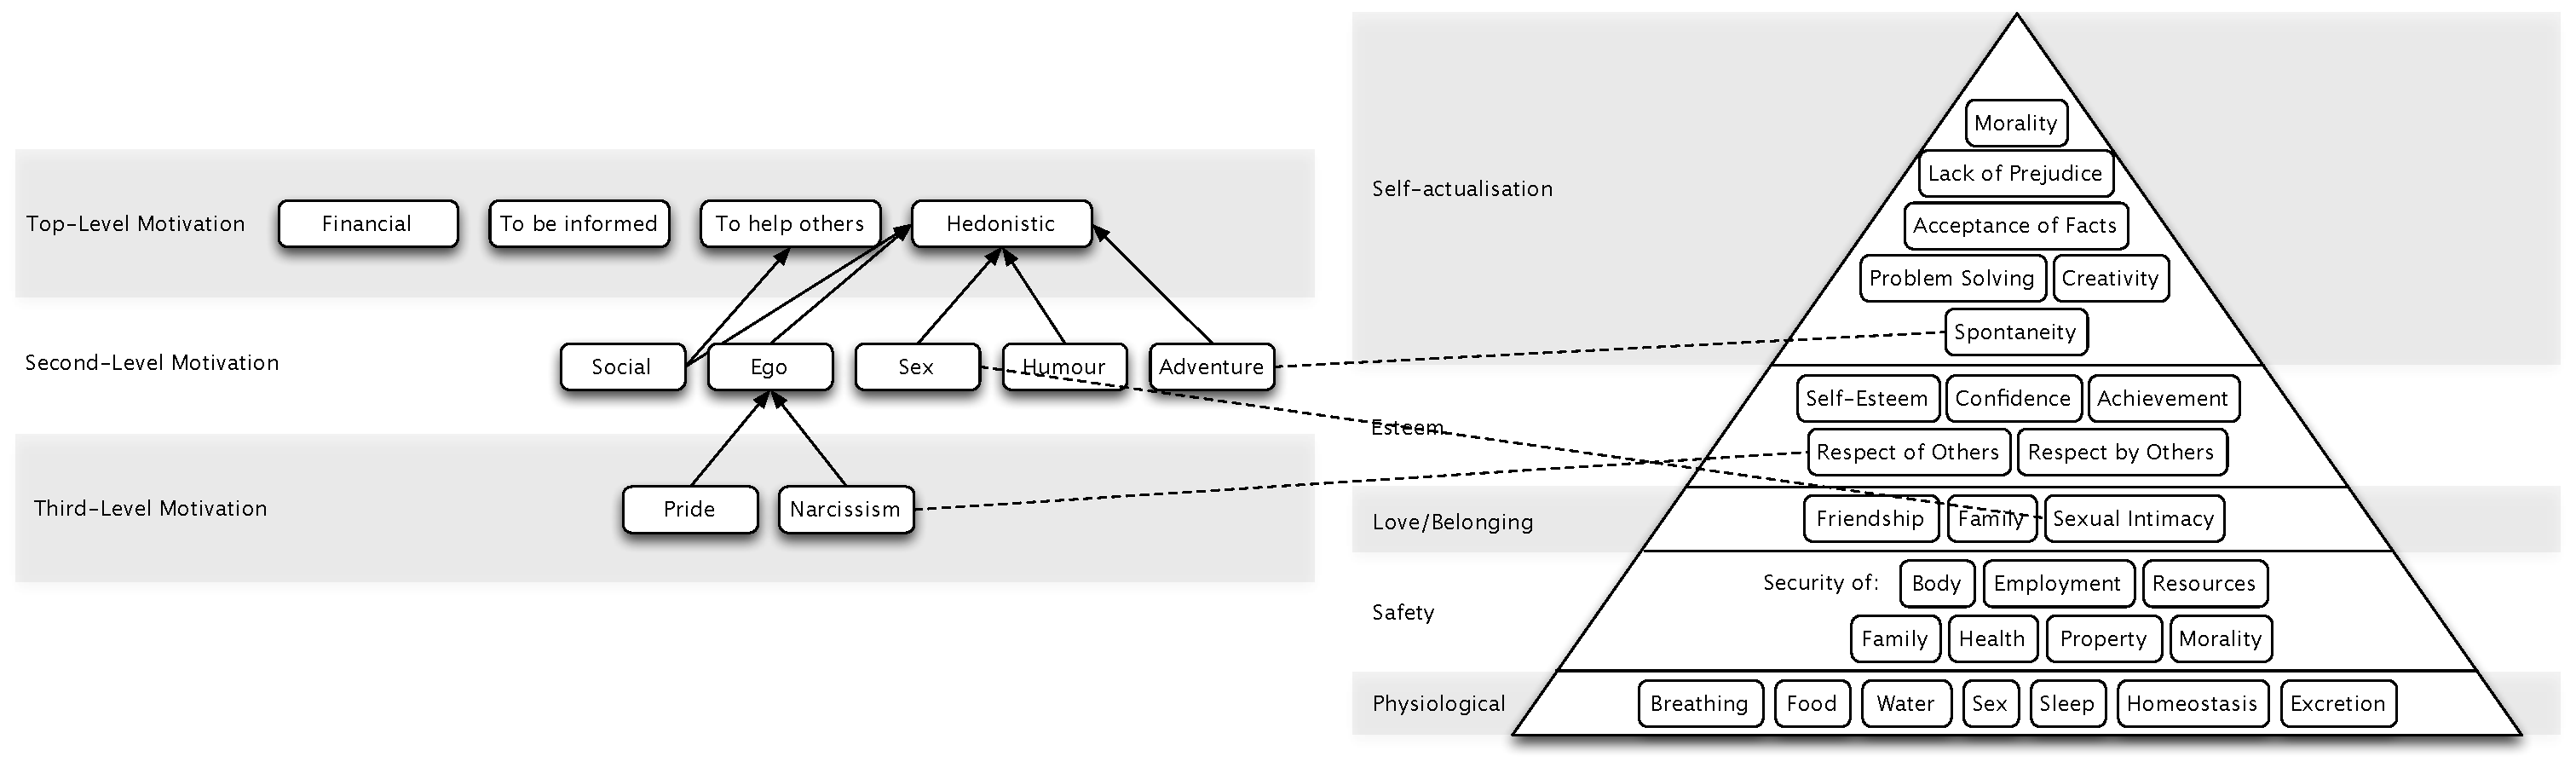
\includegraphics[width=18cm]{img/motivation.pdf}
%\caption{Motivation hierarchy of participants using Social Machines, related to Maslow's hierarchy of needs.} \label{motivation}
%\end{center}
%\end{figure*}

The motivations of users can be identified and mapped to existing human needs and motivations
systems, such as Maslow's hierarchy of human needs~\cite{maslow} (e.g., self-actualisation, security
respect of others). For each of these motivations, different roles that participate may have different {\it core motivations}, such as:

\begin{enumerate}
\item Benefit to contributor
\item Benefit to moderator
\item Benefit to system operator/host (e.g, Google, Facebook, Amazon)
\item To affiliates of the host (e.g., Amazon affiliates, YouTube partners)
\item To society as a whole
\item To a contributor's social network
\end{enumerate}

In addition to relationships to Maslow's hierarchy of needs, which drive the motivations,
we suggest that there are also resulting actions from each motivation. Thus, it should be
possible to follow basic human needs to motivations in social machines, through to the
actual actions (and therefore the necessary software feature support) that are made by
participants in social machines. Our theory is that this path may enable designers of
social machines to satisfy human needs by implemented specific features into their social
machines, or to identify potential gaps in their serving of needs and motivations due
to lack of implemented features.

Motivation in specific social machines has been studied, including motivation of participants
in: Wikipedia~\cite{kuznetsov2006motivations}; Open Source Software~\cite{lakhani2003hackers};
Peer-to-peer filesharing~\cite{p2p}; Tagging~\cite{tagging}; and Virtual
Communities~\cite{ardichvili2003motivation,Moore:2007:UMM:1235000.1235035}.

[relate this work back to ours briefly.]


\subsubsection{Artefacts of Social Machines}

Our next observation was that there are a number of shared artefact types that can be classified within the context of social machines. Specifically that
there are ``intentions'' that motivate the use of social machines, ``actions'' that are directly performed by participants of social machines, and ``contributions``
that result from the use of social machines. We have taken these abstract concepts, and mapped them to a number of well-known social machines in order
to demonstrate that these concepts can be used to compare and contrast different machines.

[more here]


\subsubsection{Metrics of participants and usage}

Finally, we identified several constructs that are relevant for all social machines. First, there are construct that relate to ``analytics'' that can be measured at a point in time, and may change over time. We have documented these constructs in Table~\ref{table:constructs}. In the left column we list construct regarding the design affordances of the social machine. In the middle column we have a mixture of the result of how the design affordances actually were realised by the social computation, such as how users co-opted / incorporated / interpreted the constraints. Finally, in the right column we list analytical measures of social machines which are subject to change over time.


\begin{table*}[htbp]
\begin{center}
\begin{tabular}{|p{18cm}|}
\hline
{\bf Designed Affordances} \\
\hline
Domain specificity [1 - Specific / 5 - General] \\
Visibility and importance of a participants `reputation' [1 - Not important / 5- Important] \\
Explicit representation of participant reputation [1 - No Reputations / 5 - Reputations] \\
Participants can define new types of contributions [1 - Not possible / 5 - Complete freedom] \\
Degree of open source software used/created [1 - Proprietary / 5 - Entirely open source] \\
Degree of openness and availability of data created in the system (APIs/Dumps) [1 - Closed/unavailable data / 5 - Completely open data] \\
Variety of actions participants can perform [1 - Single Action / 5 - Large variety of actions] \\
\hline
{\bf Participatory Affordances} \\
\hline
Supports social interaction [1 - No social features / 5 - Large variety of social features] \\
How often a participant participates (times a day, etc) [1 - Many times a day / 5 Seldom] \\
Importance of Timely Participation [1 - Unimportant / 5 - Timely] \\
Generality of Audience [1 - Niche / 5 - General] \\
Participant anonymity [1 - No Anonymity / 5 - Complete Anonymity] \\
Participant autonomy (1 - No autonomy / 5 - Complete autonomy) \\
Quality of participant contributions [1 - Low quality / 5 - High quality] \\
Clear separation of roles/responsibilities among participants - [1 - Single role - Everyone is the same) / 5 - People assume different roles/responsibilities] \\
Extent of hierarchical organisation of roles [1 - No Hierarchy / 5 - Deep/Well-defined Hierarchy] \\
Variety of types of contributions [1 - Single Type / 5 - Large variety of types] \\
Participants are motivated by extrinsic award  [1 - Disagree / 5 - Agree] \\
Participants are intrinsically motivated [1 - Disagree / 5 - Agree] \\
Service/Platform derives benefit from participant participation [1 - Disagree /  5- Agree] \\
Participants directly benefit from participating [1 - Disagree / 5 - Agree] \\
Participants' friends/social network benefit from participation [1 - Disagree / 5 - Agree] \\
Participation is for the benefit of a specific person/group other than the participant or platform owner [1-Disagree / 5-Agree] \\
Participation is for the benefit of society/the world at large  [1 - Disagree / 5 - Agree] \\
Participation is done to `get something done' [1-Disagree/5-Agree] \\
Participation is done `for fun' [1-Disagree/5-Agree] \\
Participation is done to exchange knowledge [1-Disagree/5-Agree] \\
Participation is done to be social [1-Disagree/5-Agree] \\
Participation is done via mobile devices [1-Never / 5 - Often] \\
Participants' (geographic) location is used by the service [1-No / 5 - Very] \\
\hline
{\bf Analytics} \\
\hline
Popularity [1 - Unpopular / 5 - Very Popular] \\
Maturity [1 - New / 5 - Mature] \\
Ratio of passive to active participants [1 - Passive / 5 - Active] \\
Number of competitors [1 - Not Many / 5 - Many] \\
Extent of global geographic coverage [1 - Highly localised / 5 - Global]\\
\hline
\end{tabular}
\end{center}
\caption{Constructs of social machines, listing affordances that are designed into machines, affordances that have resulted from use, and analytical constructs that can be measured and change over time.} \label{table:constructs}
\end{table*}%

The result is what we call `participation' constructs. These constructs arise from use of a
social machine, and are not necessarily predictable; they include:

\begin{enumerate}
\item {\bf Roles emerging in the social machine}
   \newline In addition to designed and implemented roles such as {\it moderator} and {\it administrator}, emerging roles include motivations of the participant, such as {\it trolls}, {\it spammers}, {\it domain experts}, {\it social nexus}, and {\it re-blogger}.
\item {\bf Quality of contributions}
    \newline For any social machine, the quality of contributions will vary. While some
    issues with quality can be predicted and protected against (e.g., through
    multi-user result agreement on Mechanical Turk~\cite{ipeirotis2010quality}), some
    particular issues with quality cannot always be predicted ahead of time.
\item {\bf Content of contributions}
    \newline While a system operator may design their social machine to generate specific
    types of content, participants may subvert the system in order to generate other types,
    or to concentrate on areas that were unforeseen at the time of launch, but are now seen
    as useful to the operators. It is also possible that multiple social machines can be
    combined/linked by users to further expand the types of contributions they produce.
\item {\bf Global / cultural reach}
    \newline A social machine may naturally focus on a narrow geographic area, for example
    an Ushahidi-based social machine for local elections~\cite{meier2008crisis} or
    natural disasters~\cite{morrow2011independent}. Such machines are unlikely to be
    re-purposed by participants outside of that area. However, some machines have been
    created for a single cultural/global area, but have potential global relevance that was
    unforeseen early on. An example is the fall-off of English-language users of the
    social network ``Orkut,'' which gained significant usage elsewhere, particularly in
    Brazil.
\item {\bf Task reach --- what do people use it for?}
    \newline In addition to breaking cultural barriers, user have also shown that they can
    use social machines for tasks that were not set up by the system operators. For example
    the identification of ``Green Pea Galaxies'' using the GalaxyZoo social machine for
    astronomy~\cite{greenpea}. Users were not originally asked to identify these types, but
    a number of users identified them, and the software was modified to include them,
    resulting in their discovery as a new type of galaxy.
\item {\bf Active/Passive participation roles}
    \newline When it comes to participation in social machines, there are levels of
    participation that can be classified as being ``active'' and being ``passive.'' These
    roles may not be particularly designed into systems, but may be exhibited over time.
    Particularly noteworthy examples can be seen in news and link aggregation social
    machines such as Reddit and Digg, where users can both submit links and vote on links.
    The frequency of each of these activities can vary wildly, with a small
    minority of users controlling the links that rise to the top~\cite{digg}.
\end{enumerate}

\subsection{Using the classification framework}

In order to demonstrate usage of our framework's constructs, we ranked our social machines
by their Alexa ranking, and performed a full repertory grid elicitation exercise over them.
This process involved ranking each social machine against the constructs, rating each construct
from 1 to 5. In total, 680 ranking were made, and the
results are illustrated in a grid and accompanying dendrograms for element and construct
similarity in Figure~\ref{dendrogram}.

\begin{figure}
\begin{center}
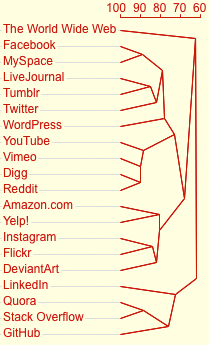
\includegraphics[width=4cm]{img/dendrogram-elements.png}
\caption{Dendrogram of elements (social machines) from a repertory grid exercise of the top 20 (ranked by Alexa) social machines from our element set, against our consolidated constructs.} \label{dendrogram}
\end{center}
\end{figure}

\begin{figure}
\begin{center}
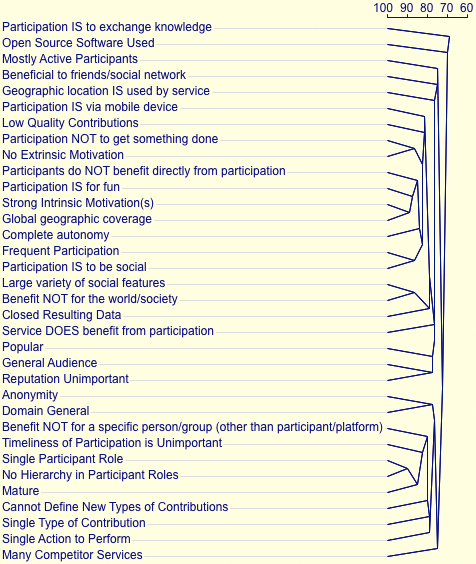
\includegraphics[width=8cm]{img/dendrogram-constructs.png}
\caption{Dendrogram of constructs from a repertory grid exercise of the top 20 (ranked by Alexa) social machines from our element set, against our consolidated constructs.} \label{dendrogram}
\end{center}
\end{figure}

From the dendrograms we can get a sense of similarities and separation of social machines. For
instance, it is clear that YouTube, Vimeo, Reddit and Digg are similar, which is logical, because
they are all social machines that focus on sharing content. Likewise, Quora and StackOverflow
are also similar, and again, this makes sense, because they are both question answering social
machines. There is also a dendrogram for the constructs, to show correlations between them. This
dendrogram indicates that there is a correlation between the ``Single Participant Roles'' and
``No Hierarchy in Participant Roles'' constructs, which is because they refer to the same
aspect of social machines. Another, but less obvious similarity is between the ``Large variety of
social features'' and ``Benefit NOT for the world/society'', which indicates that of the social
machines we have rated, there is a correlation between social features and social machines that
do not benefit the world at large, and vice-versa.

We envisage two key initial uses for this framework: for classifying social machines; and for
predicting behaviour of new/future social machines. For classifying social machines, it will
enable direct comparisons to be made with existing machines, as well as provide a platform
for discussions about social machines. We also think that the data from a large-scale classification
exercise may be useful for researchers who wish to apply prediction techniques (such as SVMs)
to social machines, their behaviour and impact.


\section{Future work: building a social machine around the classification framework}




\section{Acknowledgments}

This work is supported under SOCIAM: The Theory and Practice of Social Machines.  The SOCIAM Project is funded by the UK Engineering and Physical Sciences Research Council (EPSRC) under grant number EP/J017728/1 and comprises the Universities of Southampton, Oxford and Edinburgh.

%
% The following two commands are all you need in the
% initial runs of your .tex file to
% produce the bibliography for the citations in your paper.
\bibliographystyle{abbrv}
\bibliography{sigproc}  % sigproc.bib is the name of the Bibliography in this case
% You must have a proper ".bib" file
%  and remember to run:
% latex bibtex latex latex
% to resolve all references
%
% ACM needs 'a single self-contained file'!
%
%APPENDICES are optional


\balancecolumns % GM June 2007
% That's all folks!
\end{document}
